\documentclass[tikz,border=10pt]{standalone}
\begin{document}
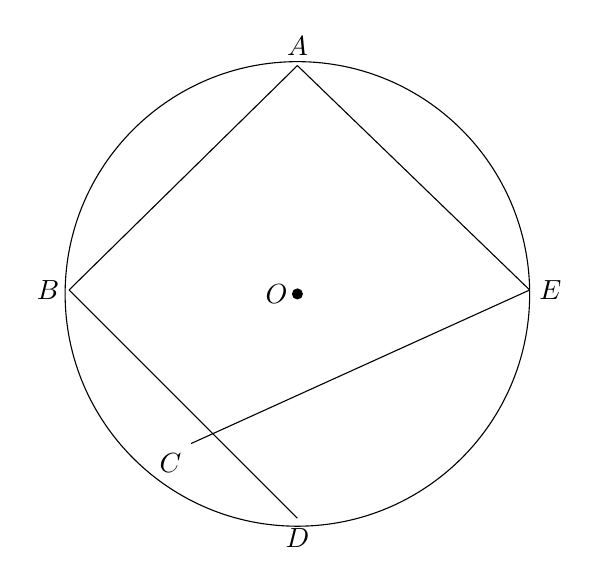
\begin{tikzpicture}[scale=1]

% Points
\coordinate (O) at (0,0);
\coordinate (A) at (0,2.9);
\coordinate (B) at (-2.9,0.05);
\coordinate (E) at (2.95,0.05);
\coordinate (D) at (0,-2.85);
\coordinate (C) at (-1.35,-1.9);

% Circle
\draw (O) circle[radius=2.95];

% Chords / segments
\draw (B) -- (A);
\draw (A) -- (E);
\draw (B) -- (D);
\draw (C) -- (E);

% Center point
\fill (O) circle[radius=2pt];

% Labels
\node[above] at (A) {$A$};
\node[left] at (B) {$B$};
\node[right] at (E) {$E$};
\node[below] at (D) {$D$};
\node[below left] at (C) {$C$};
\node[left] at (O) {$O$};

\end{tikzpicture}
\end{document}
